\chapter{Equalizer GPU Implementation}
\label{chap:equalizers_in_gpus}
Each equalizer in the PAQ presents an interesting challenge from a GPU implementation perspective.
The equations for each equalizer in Section \ref{sec:equalizer_eq} were reformulated in preparation for fast and efficient GPU implementation.
This chapter is explain how the FIR equalizer filter coefficients are computed and applied.

Every equalizer filter is computed using batch processing.
In batch processing, each packet is totally independent of all other packets.
To simplify figures, every block diagram in this chapter shows how one packet is processed.
Each packet in a batch is processed exactly the same way with different data.
If a block diagram shows how to compute one equalizer filter, the block diagram is repeated $3104$ times compute a full batch of equalizer filters.

Convolution is used many times in this chapter.
Section \ref{sec:batched_convolution} showed that GPU frequency-domain batch convolution performs best for the PAQ system.
To simplify block diagrams, frequency-domain batch convolution is shown as one block.
Figures \ref{fig:Conv2} and \ref{fig:Conv3} show how frequency-domain batch convolution is represented in this chapter.
Note that the FFT of the ``numerically optimized'' detection filter $\mathbf{H}_\text{NO}$ and the SOQPSK-TG power spectrum $\mathbf{\Psi}$ are pre-computed and do not require an additional FFT block.
\begin{figure}
	\centering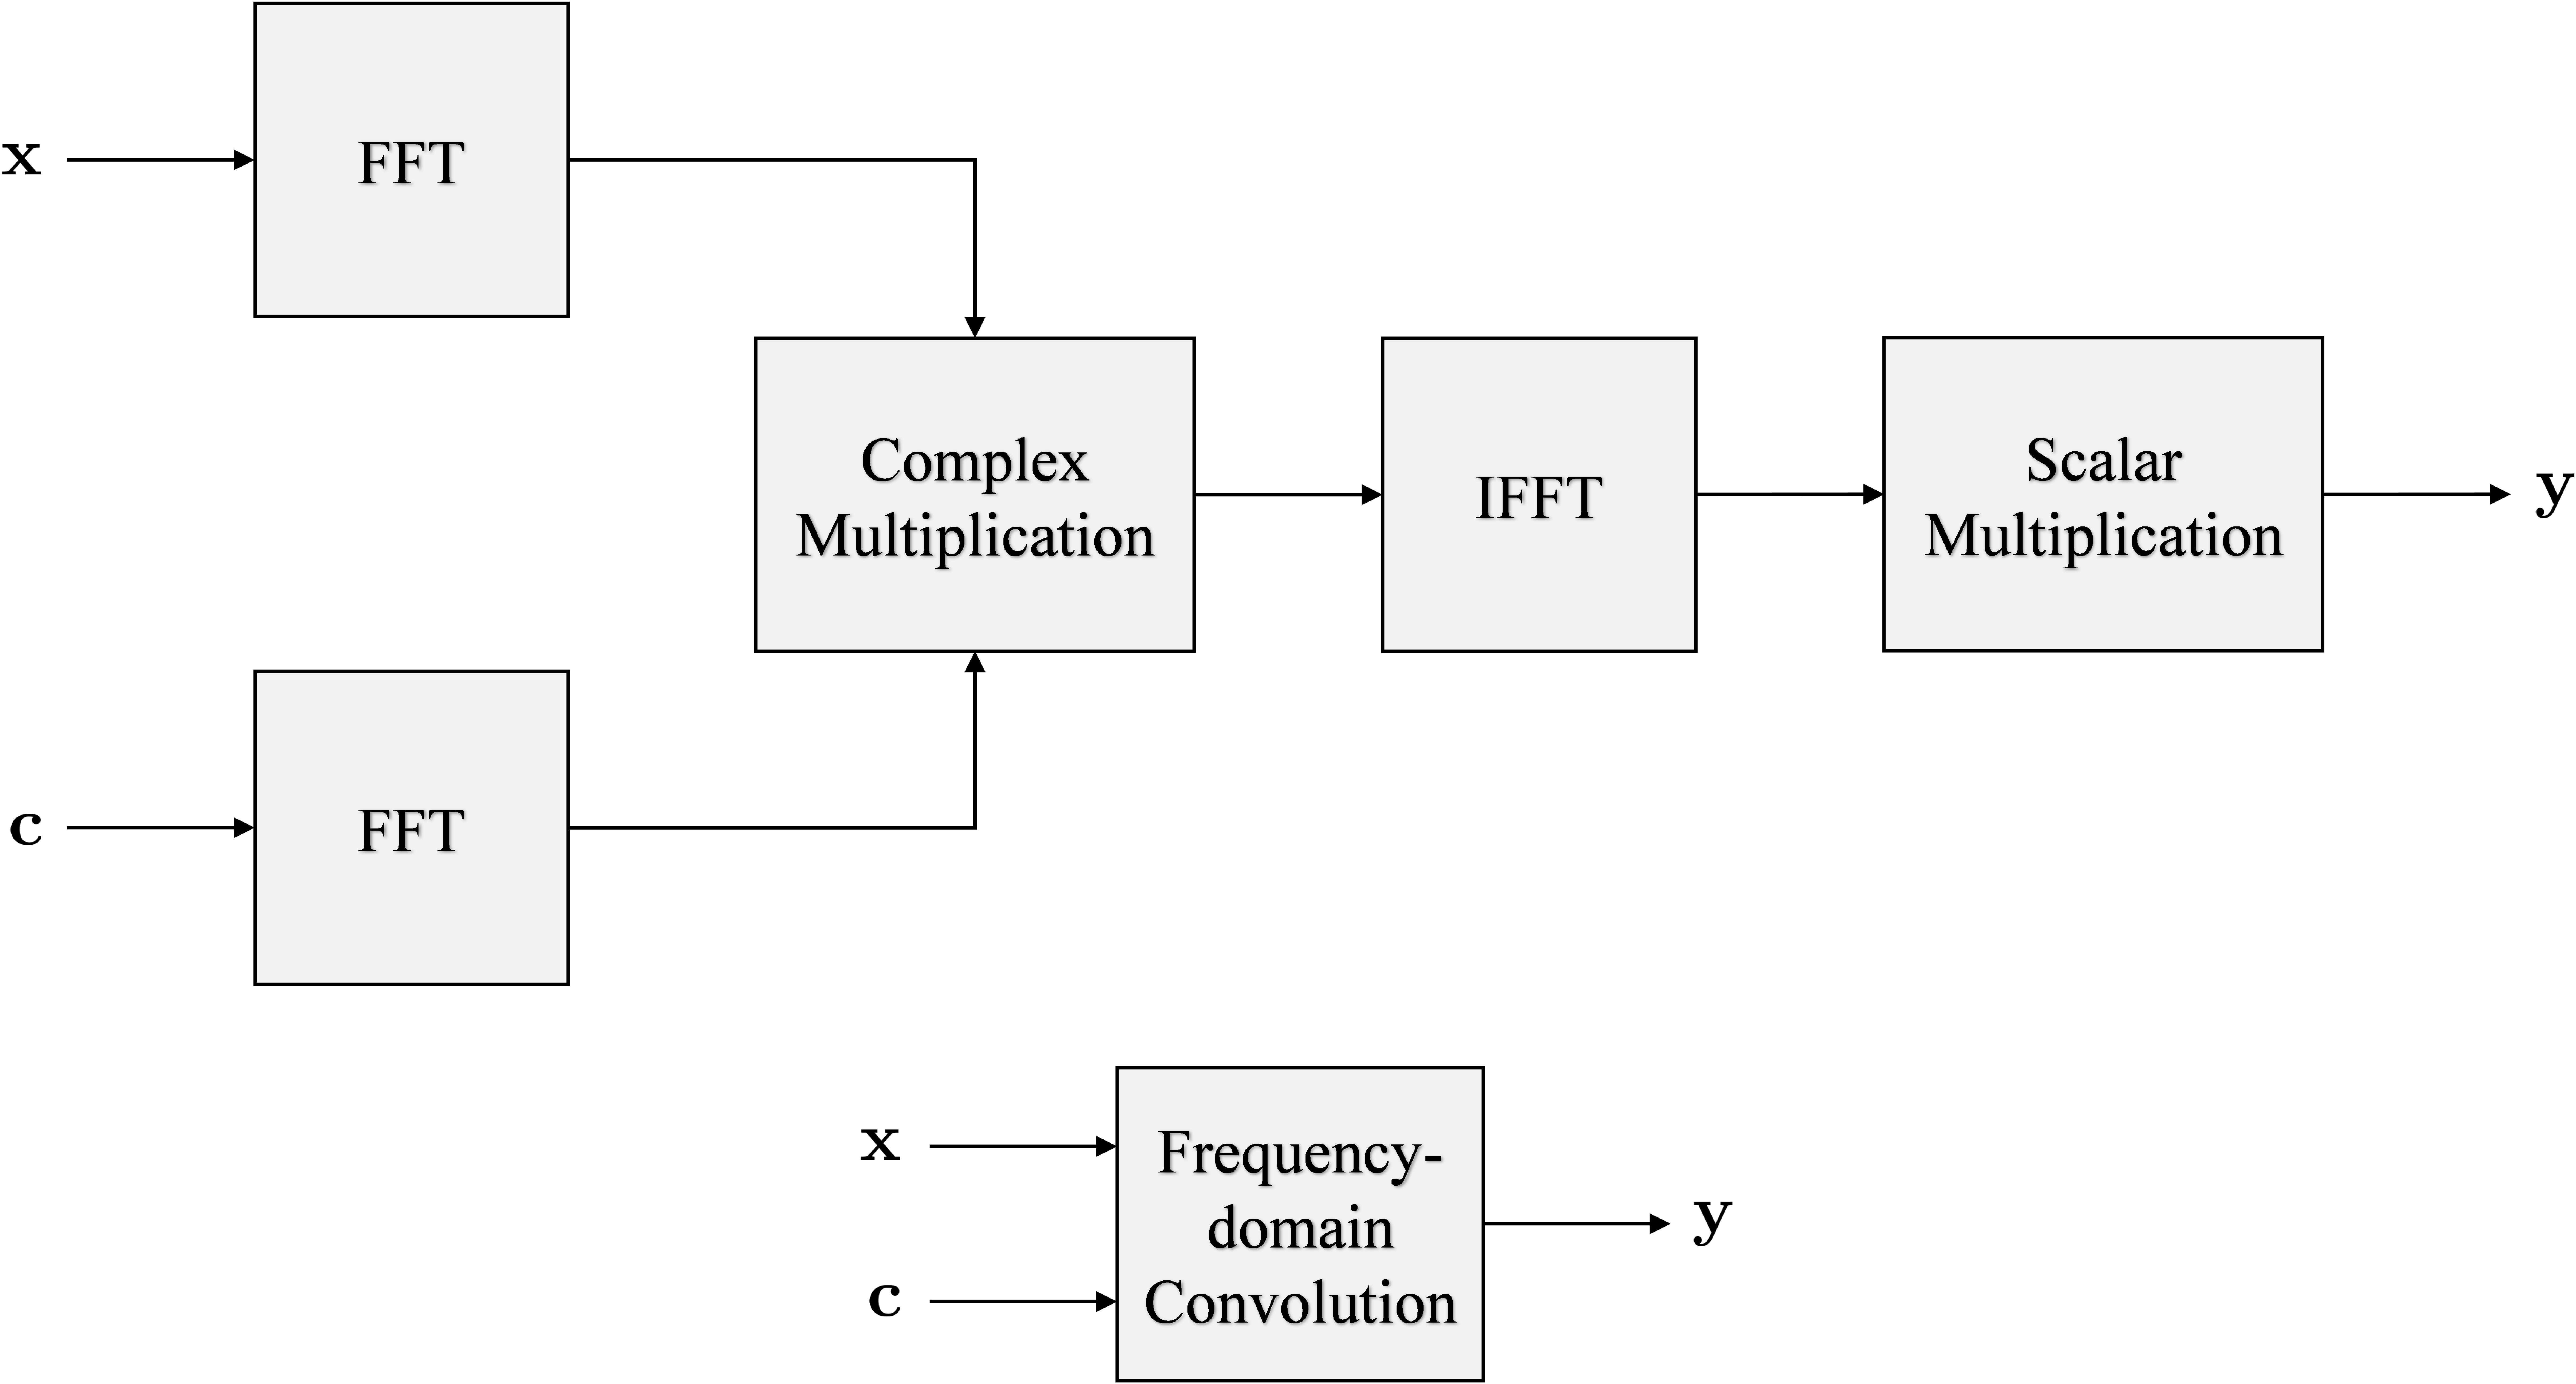
\includegraphics[width=10.28in/100*55]{figures/eq_GPUimplementation/Conv2.pdf}
	\caption{To simplify block diagrams, frequency-domain convolution is shown as one block.}
	\label{fig:Conv2}
\end{figure}
\begin{figure}
	\centering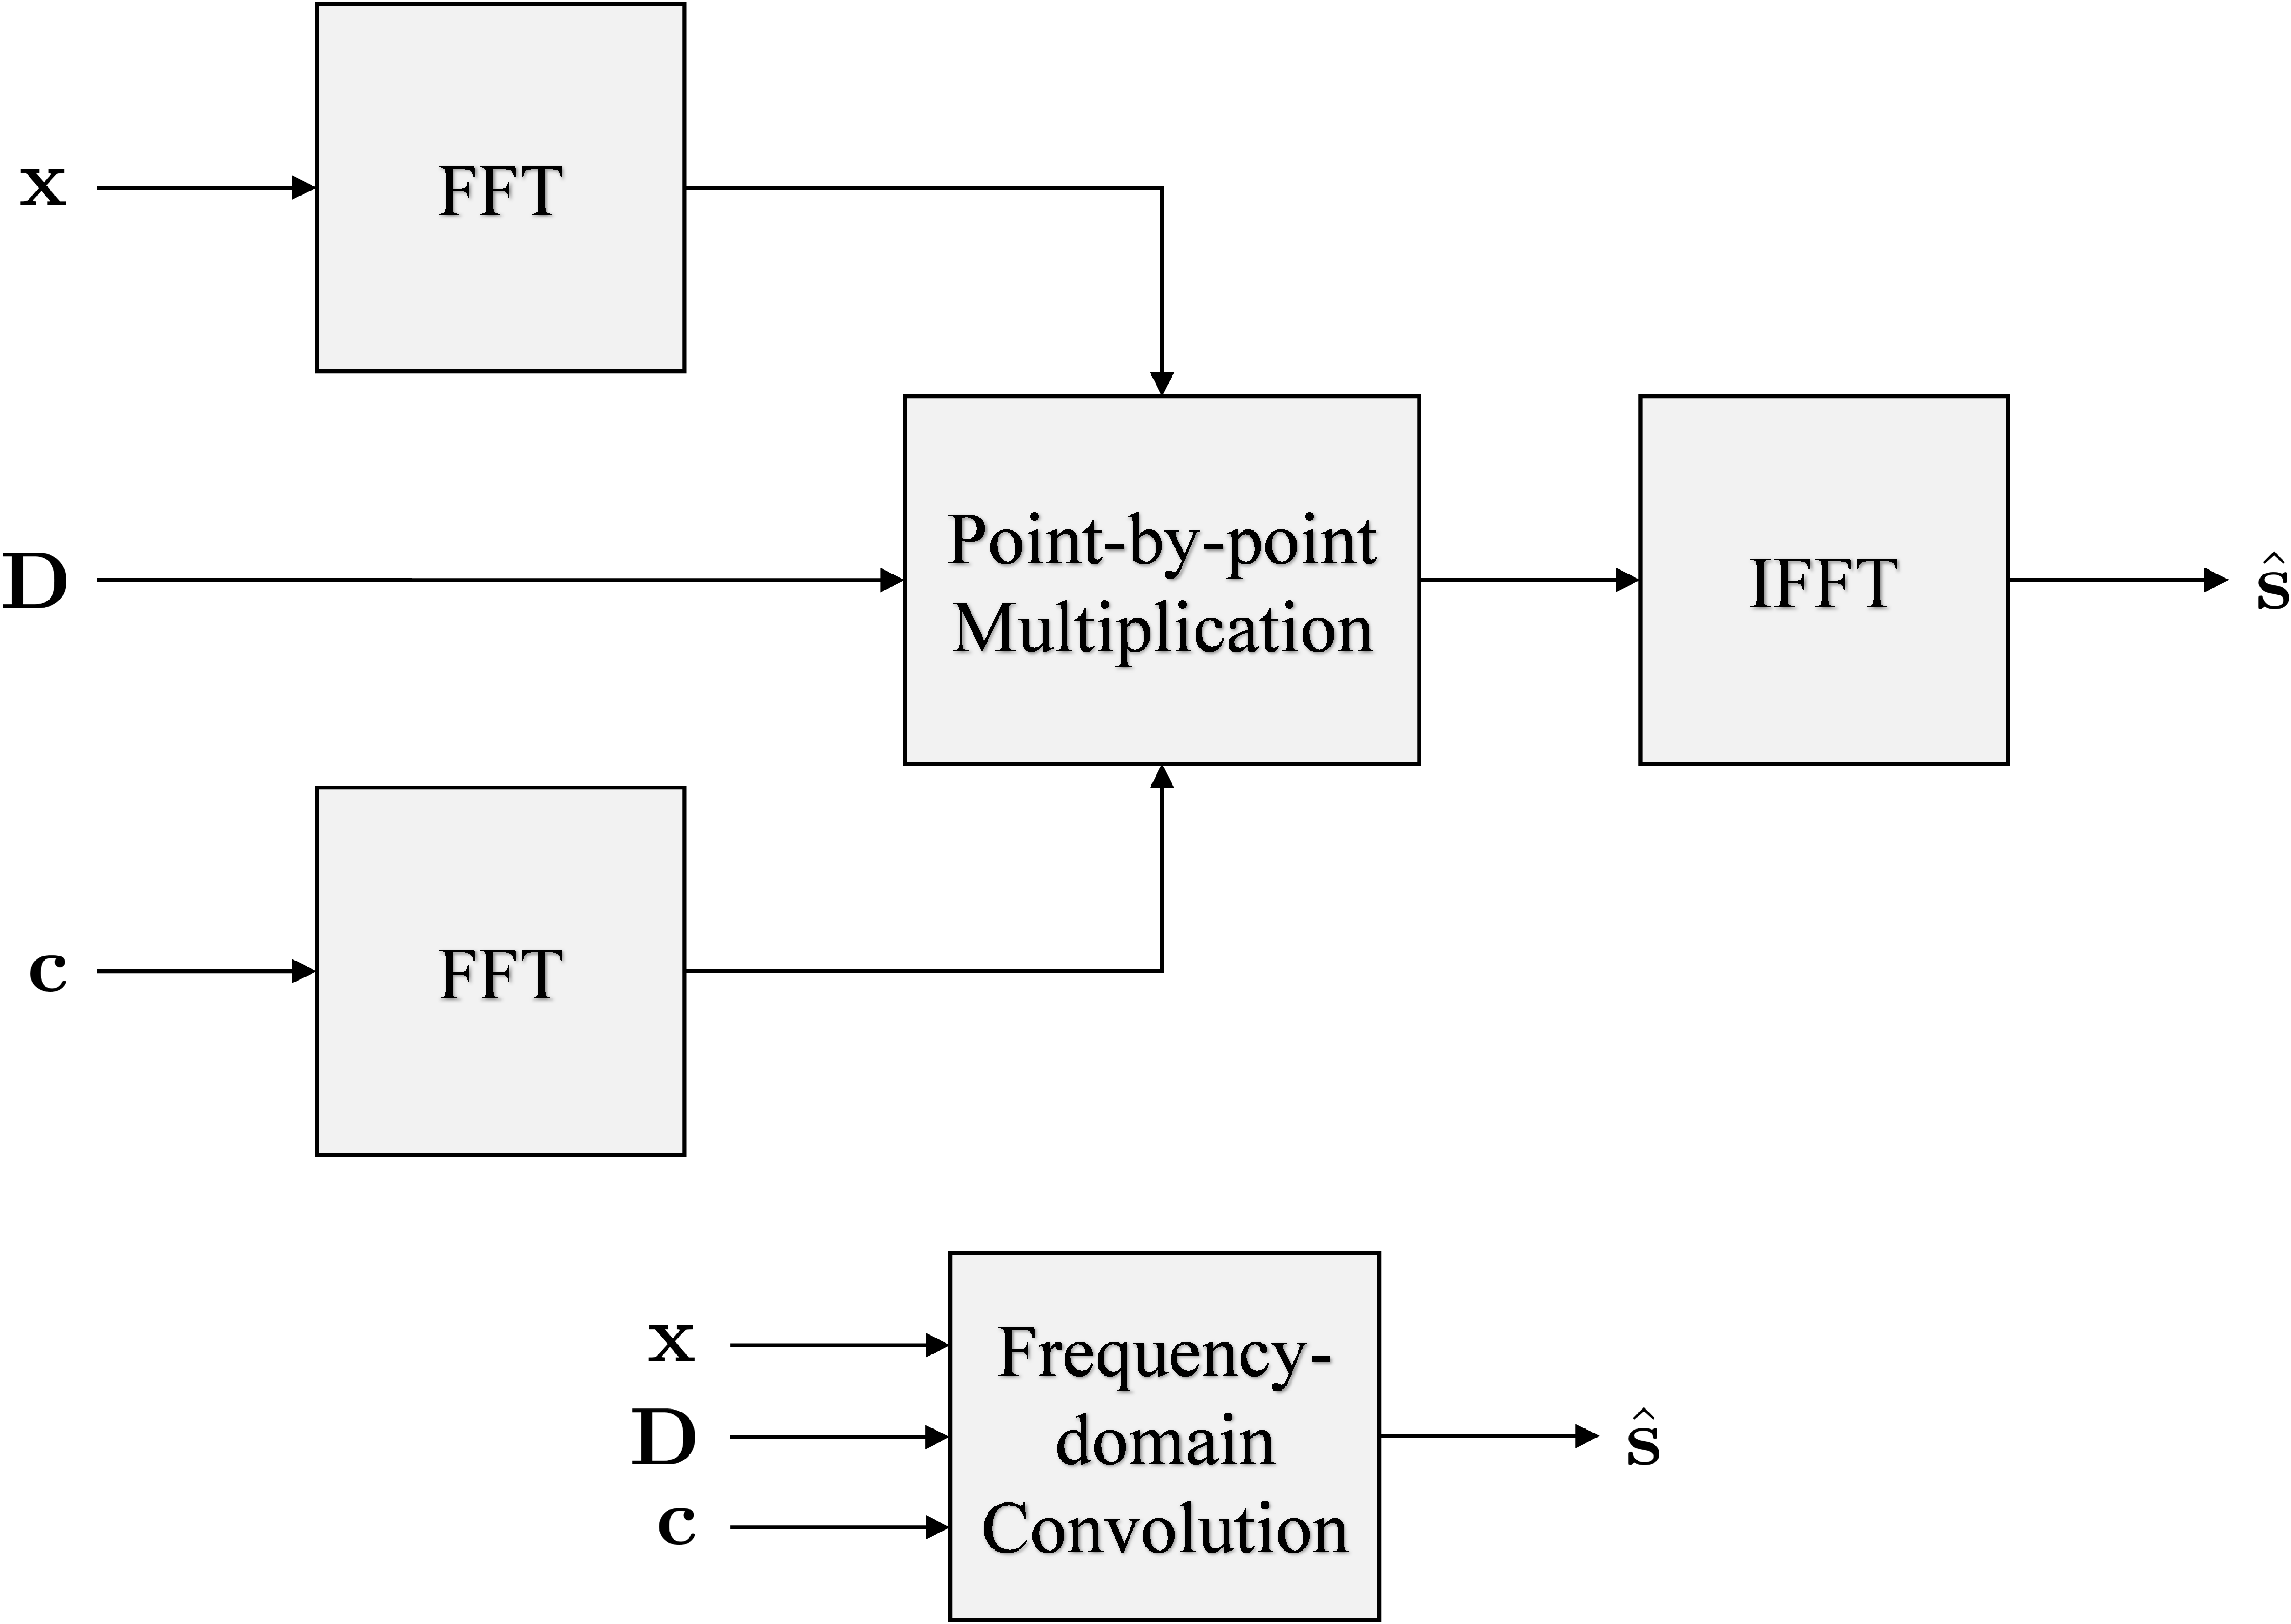
\includegraphics[width=10.28in/100*55]{figures/eq_GPUimplementation/Conv3.pdf}
	\caption{To simplify block diagrams, frequency-domain cascaded convolution is shown as one block.}
	\label{fig:Conv3}
\end{figure}

\clearpage
\section{Zero-Forcing and MMSE GPU Implementation}
The ZF and MMSE FIR equalizer filter coefficient computations have exactly the same form as shown in Equations \eqref{eq:c_ZF_solve} and \eqref{eq:c_MMSE_solve}. For reference, the equations are 
\begin{equation}
\mathbf{R}_{\hat{h}} \mathbf{c}_\text{ZF} = \hat{\mathbf{h}}_{n_0} \quad \text{or} \quad \mathbf{c}_\text{ZF} = \mathbf{R}_{\hat{h}}^{-1}\hat{\mathbf{h}}_{n_0}
\label{eq:ZF_gpuimp_solve}
\end{equation}
\begin{equation}
\mathbf{R} \mathbf{c}_\text{MMSE} = \hat{\mathbf{h}}_{n_0} \quad \text{or} \quad \mathbf{c}_\text{MMSE} = \mathbf{R}^{-1} \hat{\mathbf{h}}_{n_0}
\label{eq:MMSE_gpuimp_solve}
\end{equation}
where $\mathbf{c}_\text{ZF}$, $\mathbf{c}_\text{MMSE}$ and $\hat{\mathbf{h}}_{n_0}$ are $186\times1$ vectors and  $\mathbf{R}$ and $\mathbf{R}_{\hat{h}}$ are $186\times186$ matrices.
The only difference between ZF and MMSE is the matrix $\mathbf{R} = 
\mathbf{R}_{\hat{h}} + 2\hat{\sigma^2_w} \mathbf{I}_{L_1+L_2+1}$.

Before solving Equations \eqref{eq:ZF_gpuimp_solve} or \eqref{eq:ZF_gpuimp_solve}, $\mathbf{R}_{\hat{h}}$, $\mathbf{R}$ and $\hat{\mathbf{h}}_{n_0}$ need to be computed given $\hat{\mathbf{h}}$.
The matrices $\mathbf{R}_{\hat{h}}$ and $\mathbf{R}$ require the sample auto-correlation of the estimated channel $\mathbf{r}_{\hat{h}}$.
$\hat{\mathbf{h}}_{n_0}$ is the channel estimate time reversed and shifted.

The equalizer filters can be computed by either solving the linear system for $\mathbf{c}_\text{ZF}$ and $\mathbf{c}_\text{MMSE}$ or by computing the inverse of $\mathbf{R}$ and $\mathbf{R}_{\hat{h}}$ then performing a matrix vector multiplication.
Both techniques require $\mathcal{O}(n^3)$ operations making the computation of the ZF and MMSE equalizer filter coefficients extremely heavy.
Computing a matrix inverse or solving linear systems in GPUs is especially challenging because common algorithms are serial.
Three approaches to computing the equalizer filter coefficients was explored
\begin{itemize}
\item Levinson-Durbin recursion to solve the system of equations
\item using the cuBLAS LU decomposition library to compute the inverse and matrix vector multiplication
\item Using the cuSolver library to solve the system of equations.
\end{itemize}

Levinson-Durbin recursion avoids $\mathcal{O}(n^3)$ operations by using the Toeplitz or diagonal-constant structure of $\mathbf{R}_{\hat{h}}$ and $\mathbf{R}$ \cite[Chap. 5]{hayes:1996}.
To begin implementing Levinson-Durbin recursion, a custom GPU kernel was designed for 32-bit \textit{real} floating point data by computing $3104$ packets of ZF and MMSE equalizer filter coefficients.
Levinson-Durbin recursion showed promise by executing on real data in $500$ ms.
The algorithm was then tested on 32-bit \textit{complex} floating point data by computing $3104$ packets of  float ZF and MMSE equalizer filter coefficients.
Levinson-Durbin recursion was eliminated because execution time for complex filter coefficients was $2500$ ms.
All processing must be completed in $1907$ ms.

The next algorithm explored was computing the inverse of $\mathbf{R}_{\hat{h}}$ and $\mathbf{R}$ using the batch processing cuBLAS library. 
The cuBLAS library computes a \textit{complex} 32-bit floating point inverse using LU decompositing in $600$ ms.
cuBLAS executed faster than Levinson-Durbin recursion but $600$ ms is still $\%31$ of the total $1907$ ms processing time.

The final and fastest algorithm explored solves the linear system using the batch processing cuSolverSp library.
``cusolverSpCcsrqrsvBatched'' is the GPU function used from the cuSolverSp library.
cusolverSpCcsrqrsvBatched is a complex batch solver that leverages the sparse properties of $\mathbf{R}_{\hat{h}}$ and $\mathbf{R}$ by utilizing Compressed Row Storage (CRS) \cite{wiki:Sparse_matrix}.
The Compressed Row Storage reduces the large $186\times186$ matrices to $12544$ element CSR matrices $\mathbf{R}_{\hat{h}\text{CRS}}$ and $\mathbf{R}_{\text{CRS}}$.
Before cusolverSpCcsrqrsvBatched can be called, the CSR matrix $\mathbf{R}_{\hat{h}\text{CRS}}$ has to be built using $\mathbf{r}_{\hat{h}}$.
An example of how to use the CUDA cusolverSp library can be found \cite{CUDA_toolkit_doc}.

Figures \ref{fig:blockZF} and \ref{fig:blockMMSE} show how the ZF and MMSE equalizer filters are computed and applied to the received samples.
Note that the equalizer filters are applied in the frequency-domain with the detection filter.
\begin{figure}
	\centering\includegraphics[width=7.5in/100*55]{figures/eq_GPUimplementation/blockZF.pdf}
	\caption{Block Diagram showing how the Zero-Forcing equalizer coefficients are implemented in the GPU.}
	\label{fig:blockZF}
\end{figure}
\begin{figure}
	\centering\includegraphics[width=7.98in/100*55]{figures/eq_GPUimplementation/blockMMSE.pdf}
	\caption{Block Diagram showing how the Minimum Mean Squared Error equalizer coefficients are implemented in the GPU.}
	\label{fig:blockMMSE}
\end{figure}
Table \ref{tab:ZFMMSEtimingComparison} lists the algorithms researched and their respective execution times.
\begin{table}
\caption{Defining start and stop lines for timing comparison in Listing \ref{code:convFun}.}
\begin{center}
\begin{tabular}{lll}
	\toprule
	Algorithm 			& Data type	& Execution Time (ms)	\\ \midrule
	Levinson Recursion 	& floats 	& 500 					\\
	Levinson Recursion 	& Complex 	& 2500 					\\
	LU Decomposition 	& Complex 	& 600				 	\\
	cuSolver			& Complex	& 355.96				\\
	\bottomrule
\end{tabular}
\end{center}
\label{tab:ZFMMSEtimingComparison}
\end{table}

\clearpage
\section{Constant Modulus Algorithm GPU Implementation}
The Constant Modulus Algorithm (CMA) computes FIR equalizer filter coefficients by a steepest decent algorithm in Equation \eqref{eq:steepest}.
The more iterations a steepest decent algorithm executes, the better the CMA equalizer file will be.
The cost function gradient used in the steepest decent algorithm is $\nabla J$ shown in Equation \eqref{eq:DelJcma-midMassage}.
These equations are shown here for reference:
\begin{equation}
\mathbf{c}_\text{CMA($b+1$)} = \mathbf{c}_\text{CMA($b$)}-\mu \nabla J
\end{equation}
\begin{equation}
	\nabla J = \frac{1}{L_{pkt}} \sum_{n=0}^{L_{pkt}-1}
	z(n)  \mathbf{r}^\ast(n) \quad or \quad \nabla J(k) = \frac{1}{L_{pkt}} b(k), \quad -L_1 \leq k \leq L_2
	\label{eq:CMA_challenge}
\end{equation}
where
\begin{equation}
z(n) = 	2\left[ \vphantom{\displaystyle\sum}  y(n) y^\ast(n) - 1 \right] y(n),
\end{equation} 
\begin{align}
b(n) &= \sum^{L_{pkt}-1}_{m=0} z(m) \rho(n-m)
\end{align}
and
\begin{equation}
\rho(n) = r^\ast(n).
\end{equation}

The most computationally heavy portion of the CMA equalizer filter implementation is computing the cost function gradient $\nabla J$ in Equation \eqref{eq:CMA_challenge}.
Section \ref{sec:CMA} showed there is two approaches to computing $\nabla J$: directly or using convolution.

The direct approach didn't allow for multiple iterations because each equalizer filter coefficient required a $12672$ sample summation.
The summation in GPU kernels performs poorly because every equalizer filter coefficient accesses the full packet of received samples.
One CMA iteration took $421.317$ ms to execute computing $\nabla J$ directly also applying $\mathbf{c}_\text{CMA($b$)}$ and computing $\mathbf{c}_\text{CMA($b+1$)}$.

Using convolution to compute $\nabla J$ majorly decreased execution time for the CMA equalizer filter.
One CMA iteration took $88.774$ ms to execute computing $\nabla J$ using frequency-domain convolution also applying $\mathbf{c}_\text{CMA($b$)}$ and computing $\mathbf{c}_\text{CMA($b+1$)}$.
Note that all other frequency-domain convolution in this thesis $2^{14}$ or $16384$ points, but the convolution length $12672+12672-1$ is greater than $16384$. 
The FFTs in the computation of $\nabla J(k)$ are $2^{15}$ or $32768$ point FFTs.

Figure \ref{fig:blockCMA} shows a block diagram of how the CMA equalizer runs on the GPU.
Note that the detection filter is applied only on the last iteration.
Table \ref{tab:CMAtimingComparison} lists the comparison on computing $\nabla J(k)$ verse using convolution.
By reformulating the computation of $\nabla J$, the execution time was reduced by $4.74$ times.
The number of CMA iterations went from 2 iterations using direct implementations to 12 iterations using the convolution implementation.
\begin{figure}
	\centering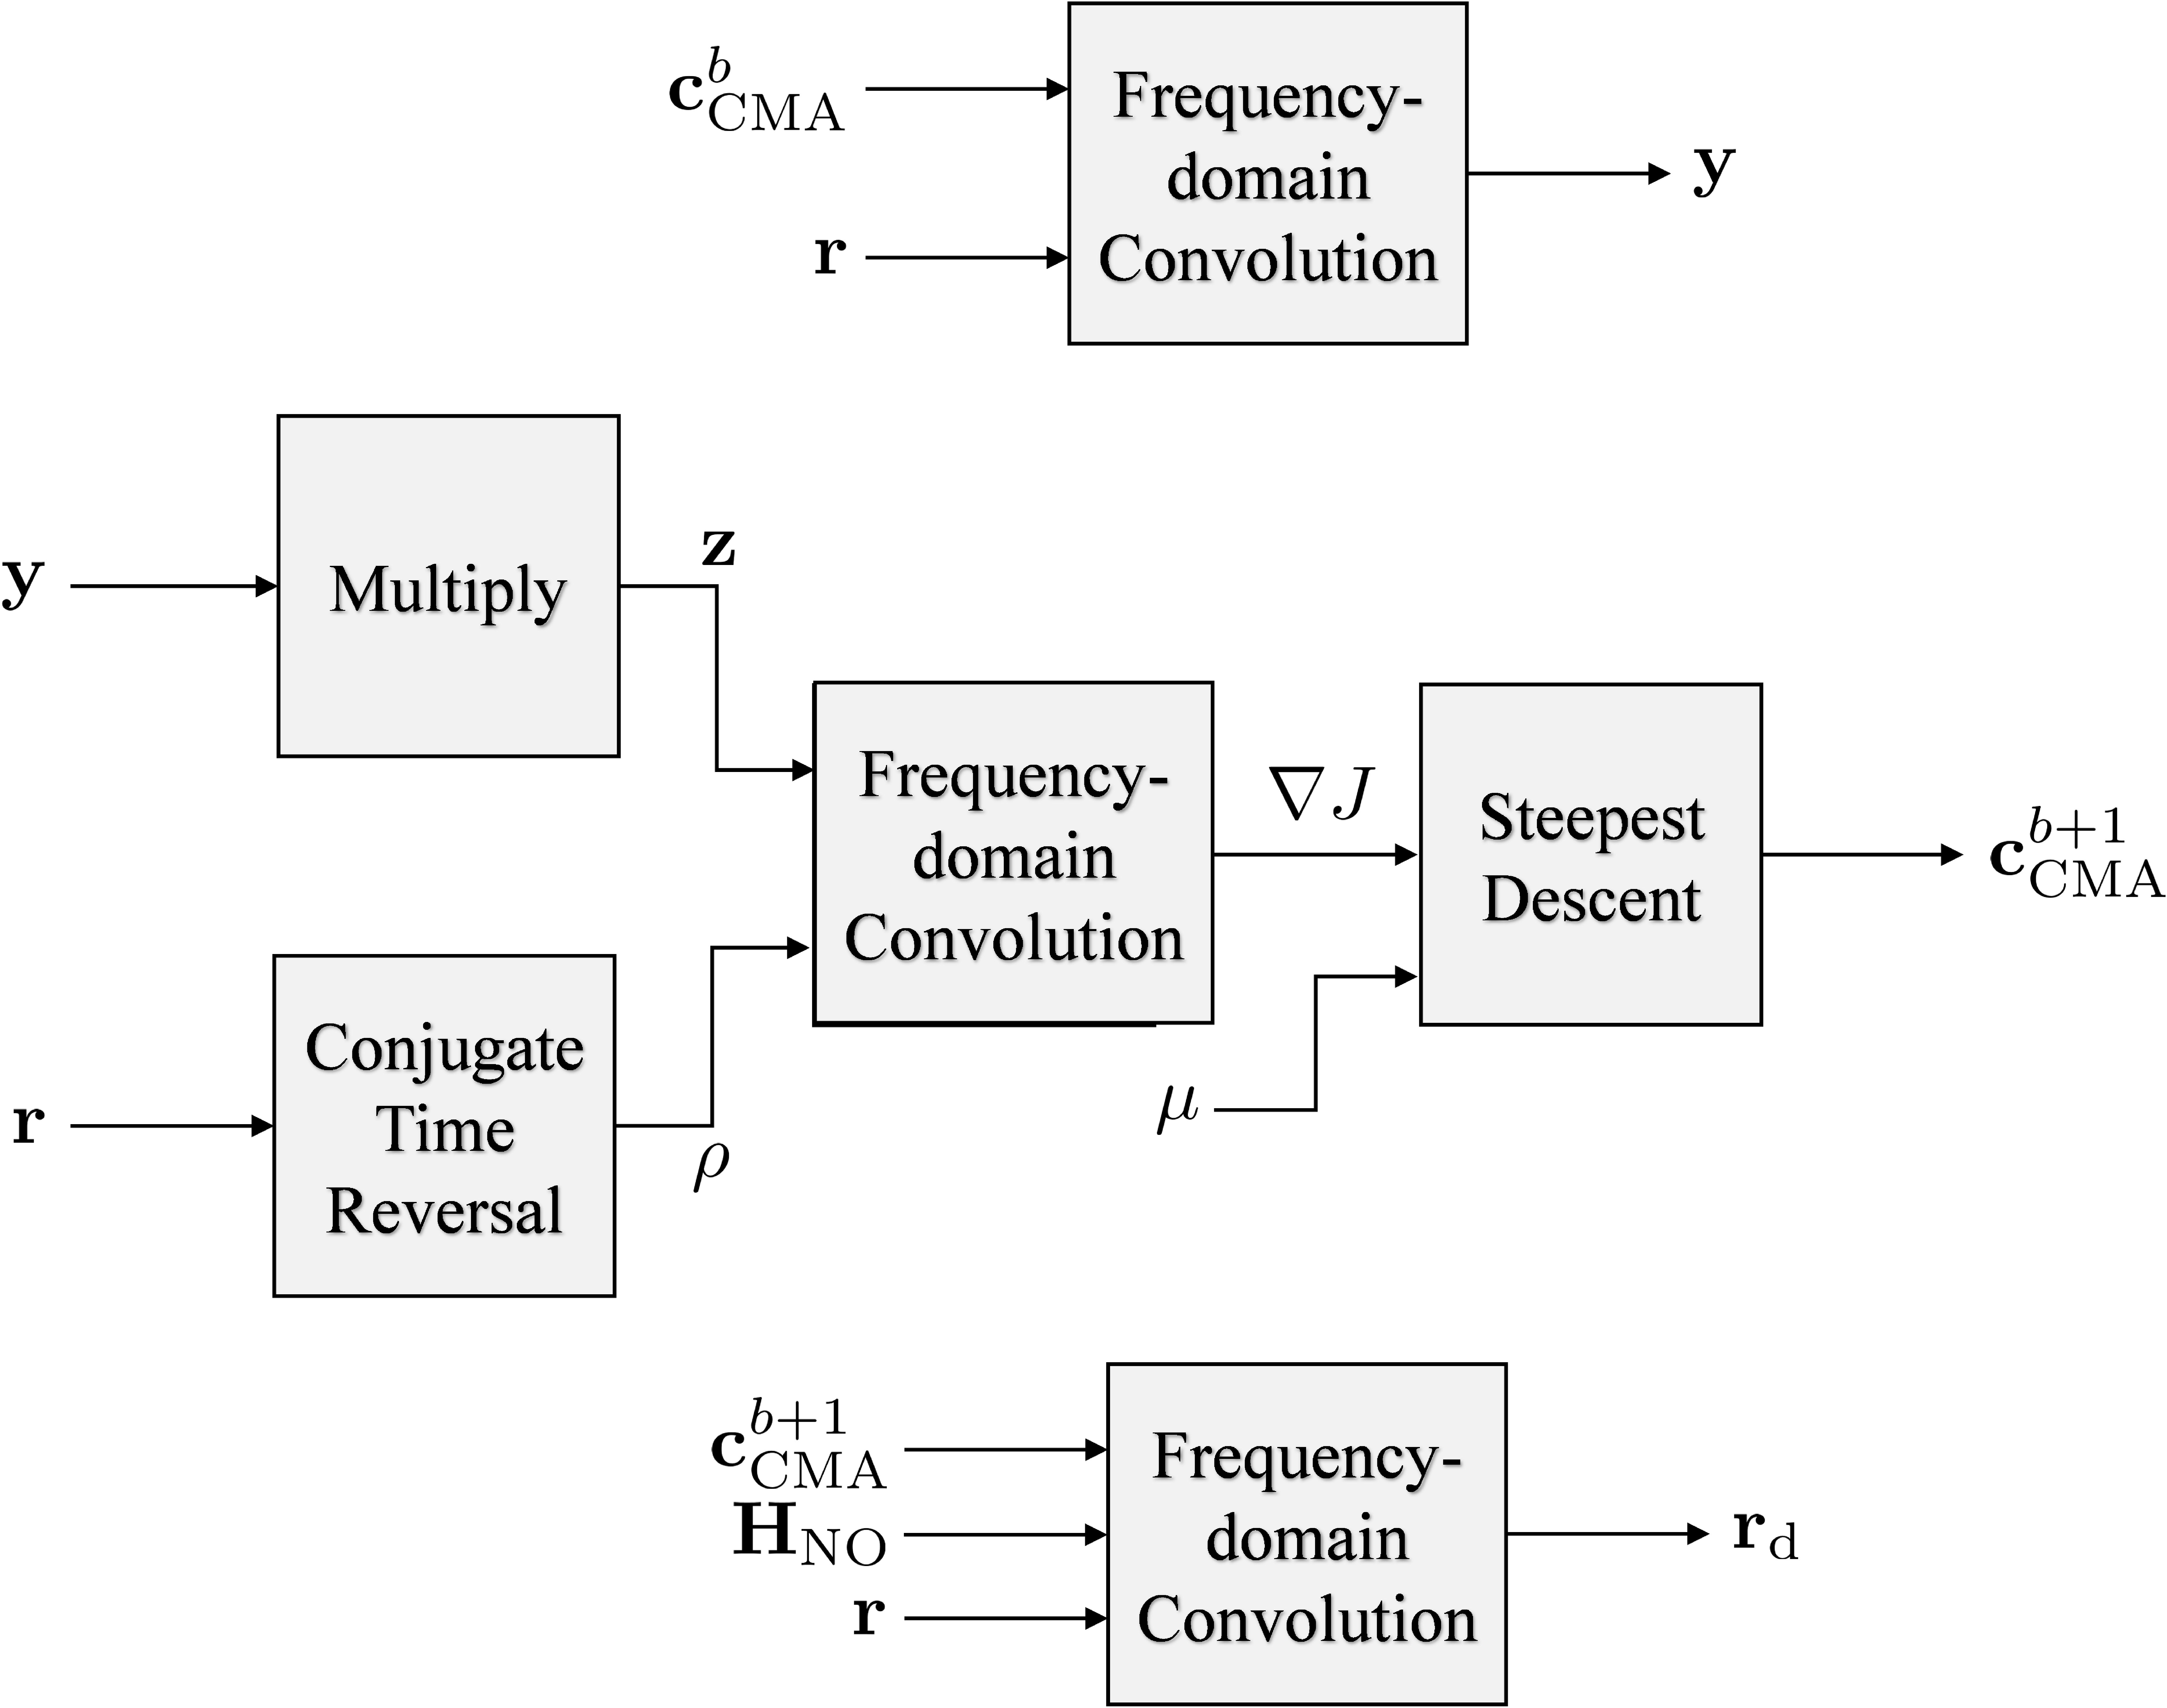
\includegraphics[width=8.34in/100*55]{figures/eq_GPUimplementation/blockCMA.pdf}
	\caption{Block Diagram showing how the CMA equalizer filter is implemented in the GPU using frequency-domain convolution twice per iteration.}
	\label{fig:blockCMA}
\end{figure}
\begin{table}
\caption{The gradient vector $\nabla J$ can be computed directly or using convolution.}
\begin{center}
\begin{tabular}{lll}
	\toprule
	CMA	Iteration Algorithm		& Execution Time (ms)	\\ \midrule
	$\nabla J$ directly 		& 421.317				\\
	$\nabla J$ using convolution & 88.774				\\
	\bottomrule
\end{tabular}
\end{center}
\label{tab:CMAtimingComparison}
\end{table}

\section{Frequency Domain Equalizer One and Two GPU Implementation}
The Frequency Domain Equalizers (FDEs) were by far the fastest and easiest to implement into GPUs.
The block diagram looks just like convolution except that complex multiplication is
\begin{equation}
R_\text{d1}(e^{j\omega_k}) = \frac{R(e^{j\omega_k}) \hat{H}^\ast(e^{j\omega_k}) H_{\text{NO}}(e^{j\omega_k})}  {|\hat{H}(e^{j\omega_k})|^2  +  \frac{1}{\hat{\sigma}^2_w}} \quad
\text{where} \;
\omega_k = \frac{2\pi}{L} \;
\text{for} \;
k=0,1,\cdots,L-1
\label{eq:FDE1_applied}
\end{equation}
or
\begin{equation}
R_\text{d2}(e^{j\omega_k}) = \frac{R(e^{j\omega_k}) \hat{H}^\ast(e^{j\omega_k}) H_{\text{NO}}(e^{j\omega_k})}  {|\hat{H}(e^{j\omega_k})|^2  +  \frac{\Psi(e^{j\omega_k})}{\hat{\sigma}^2_w}} \quad
\text{where} \;
\omega_k = \frac{2\pi}{L} \;
\text{for} \;
k=0,1,\cdots,L-1
\label{eq:FDE2_applied}
\end{equation}
where $R(e^{j\omega_k})$ and $R_\text{d}(e^{j\omega_k})$ is the FFT $\mathbf{r}$ and $\mathbf{r}_\text{d}$ 
at $\omega_k$.
Equations \eqref{eq:FDE1_applied} and \ref{eq:FDE2_applied} apply FDE1 and FDE2 from Equations \eqref{eq:FDE1} and \eqref{eq:FDE2} to the received samples and apply the detection filter.
Figures \ref{fig:blockFDE1} and \ref{fig:blockFDE2} show the block diagrams for GPU implementation.
As expected, these figures look just like the frequency-domain convolution block diagrams shown in Figures \ref{fig:Conv2} and \ref{fig:Conv3}.
Table \ref{tab:FDEtimingComparison} shows the execution times for calculating and applying FDE1 and FDE2.
\begin{table}
\caption{Execution times for calculating and applying Frequency Domain Equalizer One and Two.}
\begin{center}
\begin{tabular}{lll}
	\toprule
	Algorithm						& Execution Time (ms)	\\ \midrule
	Frequency Domain Equalizer One 	& 57.156				\\
	Frequency Domain Equalizer Two	& 58.841				\\
	\bottomrule
\end{tabular}
\end{center}
\label{tab:FDEtimingComparison}
\end{table}
\begin{figure}
	\centering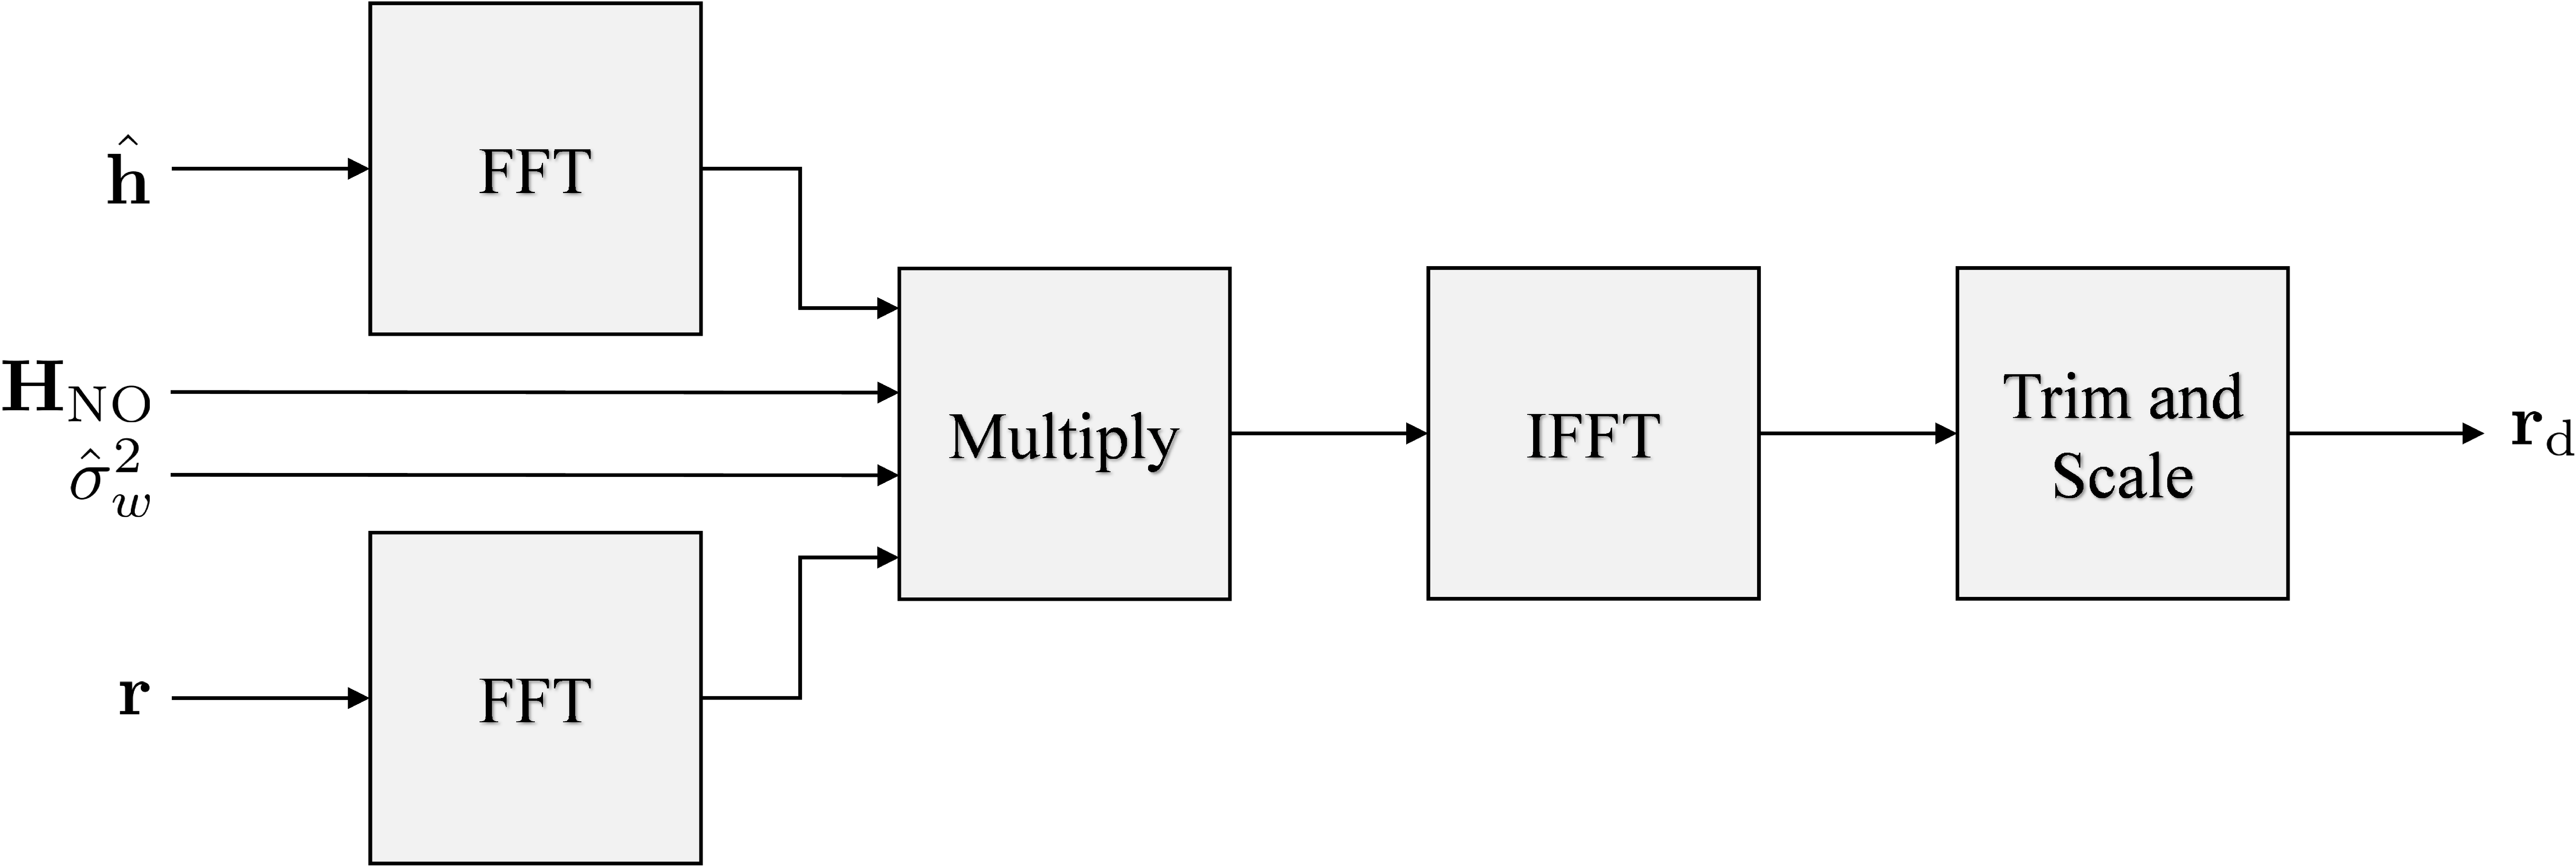
\includegraphics[width=9.73in/100*55]{figures/eq_GPUimplementation/blockFDE1.pdf}
	\caption{Diagram showing Frequency Domain Equalizer One is implemented in the frequency domain in GPUs.}
	\label{fig:blockFDE1}
\end{figure}
\begin{figure}
	\centering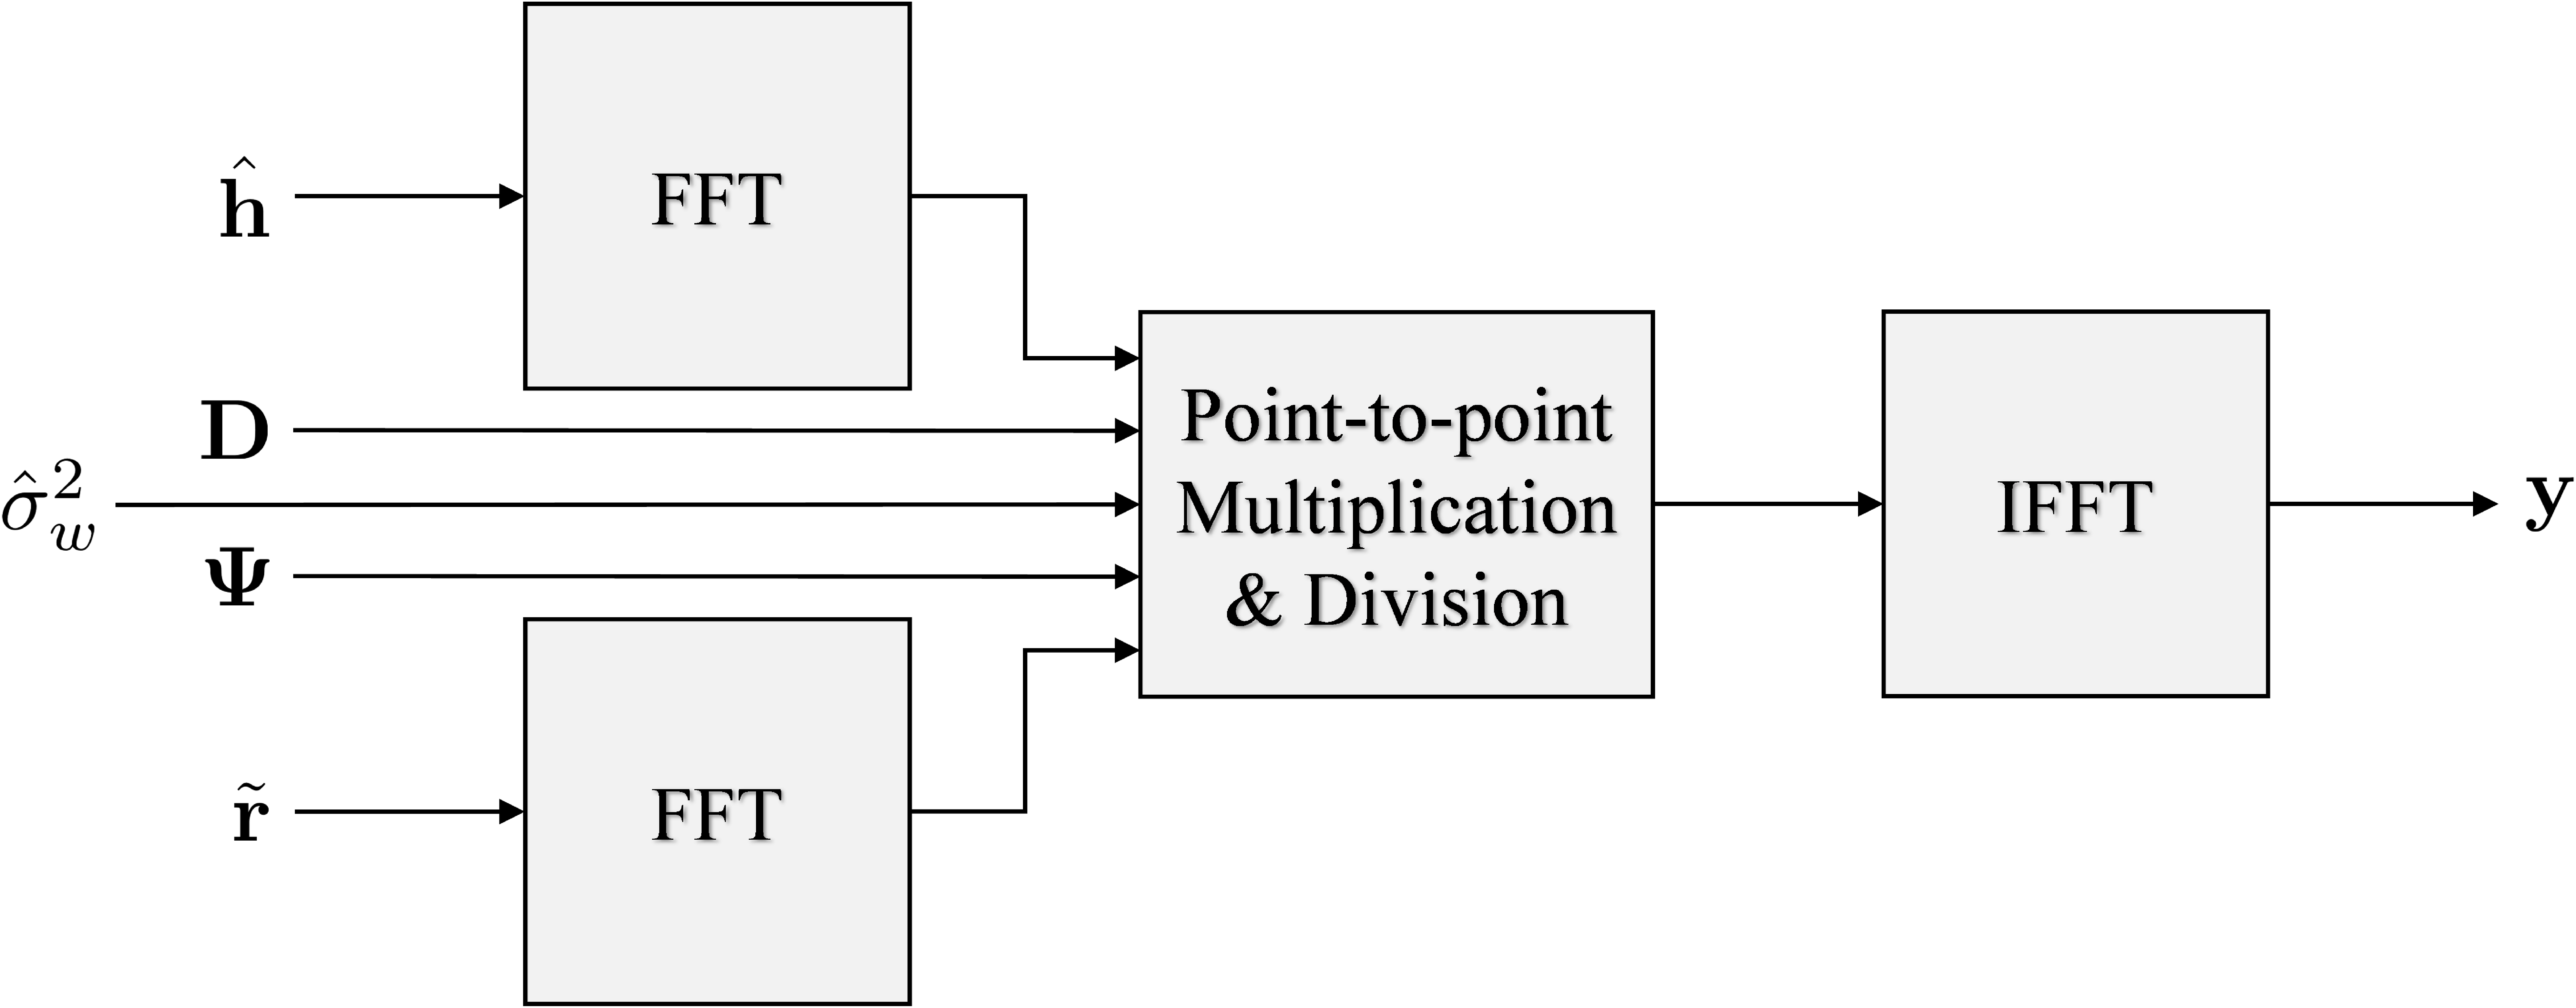
\includegraphics[width=10.03in/100*55]{figures/eq_GPUimplementation/blockFDE2.pdf}
	\caption{Diagram showing Frequency Domain Equalizer Two is implemented in the frequency domain in GPUs.}
	\label{fig:blockFDE2}
\end{figure}





